\documentclass[border=2]{standalone}
\usepackage[utf8]{inputenc}

%\usepackage{tikz} // Per a mes informacio, canviBase2aDeu.tex
%\usetikzlibrary{shapes,arrows, shadows}
\usepackage{flowchart}
\usetikzlibrary{arrows}

% la nova documentacio http://ctan.mackichan.com/graphics/pgf/contrib/flowchart/flowchart.pdf

% process/ decision/ terminal/ predproc/ storage/

\begin{document}
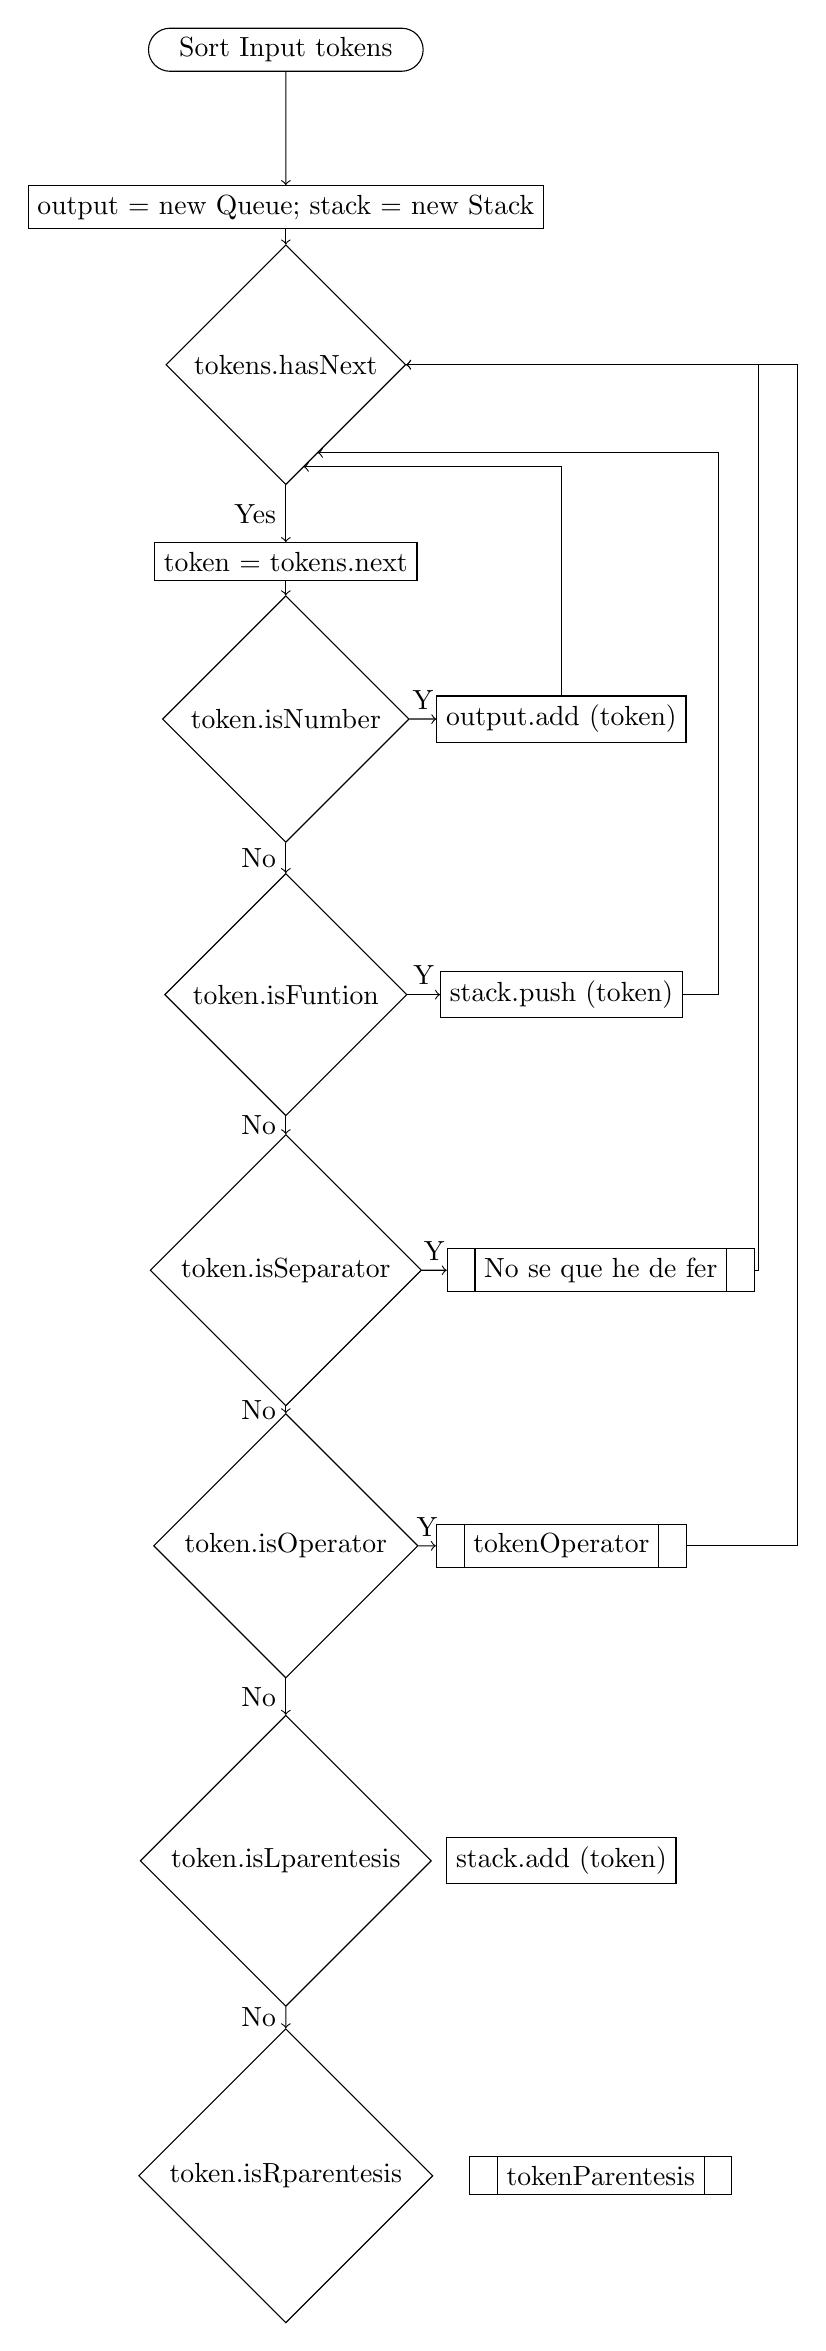
\begin{tikzpicture}[node distance = 2cm, auto]

%%%%%%%%%%%%%%%%%%%%%%%%%%%%%%%%%%%%%%%%%%%%%%%%%%%%%%%%%%%%%%%%%%%%%%%%%%%%%%%%%%%%%%%%%%%%%%%%%%%%%%%%%%%%%%%%%%%%%%%%%%%%%%%%
% Nucli, principal
%%%%%%%%%%%%%%%%%%%%%%%%%%%%%%%%%%%%%%%%%%%%%%%%%%%%%%%%%%%%%%%%%%%%%%%%%%%%%%%%%%%%%%%%%%%%%%%%%%%%%%%%%%%%%%%%%%%%%%%%%%%%%%%%
	\node [draw, terminal] (start) {Sort Input tokens};
	\node [draw, process, below of=start] (newVar) {output = new Queue; stack = new Stack};
	\node [draw, decision, below of=newVar] (mainWhile) {tokens.hasNext};
	\node [draw, process, below of=mainWhile, node distance=2.5cm] (lectura) {token = tokens.next};
	\node [draw, decision, below of=lectura] (numero) {token.isNumber};
		\node [draw, process, right of=numero, node distance=3.5cm] (fiDigit) {output.add (token)};
	\node [draw, decision, below of=numero, node distance=3.5cm] (funcio) {token.isFuntion};
		\node [draw, process, right of=funcio, node distance=3.5cm] (fiFuncio) {stack.push (token)};
% no pillo
% Until the token at the top of the stack is a left parenthesis, pop operators off the stack onto the output queue. If no left parentheses are encountered, either the separator was misplaced or parentheses were mismatched
	\node [draw, decision, below of=funcio, node distance=3.5cm] (funcioArgumentSeparador) {token.isSeparator};
		\node [draw, predproc, right of=funcioArgumentSeparador, node distance=4cm] (fiSeparador) {No se que he de fer};
	\node [draw, decision, below of=funcioArgumentSeparador, node distance=3.5cm] (operacio) {token.isOperator};
		\node [draw, predproc, right of=operacio, node distance=3.5cm] (fiOperacio) {tokenOperator};
	\node [draw, decision, below of=operacio, node distance=4cm] (openParentesis) {token.isLparentesis};
		\node [draw, process, right of=openParentesis, node distance=3.5cm] (fioParentesis) {stack.add (token)};
	\node [draw, decision, below of=openParentesis, node distance=4cm] (rightParentesis) {token.isRparentesis};
		\node [draw, predproc, right of=rightParentesis, node distance=4cm] (fiRparentesis) {tokenParentesis};
% fletxes
\draw[->] (start)	-- (newVar);
\draw[->] (newVar)	-- (mainWhile);
\draw[->] (mainWhile)	-- node[anchor=east] {Yes} (lectura);
\draw[->] (lectura)	-- (numero);
\draw[->] (numero)	-- node[anchor=east] {No} (funcio);
	\draw[->] (numero)	-- node[anchor=south] {Y} (fiDigit);
	\draw[->] (fiDigit) |- (mainWhile.-80);
\draw[->] (funcio)	-- node[anchor=east] {No} (funcioArgumentSeparador);
	\draw[->] (funcio)	-- node[anchor=south] {Y} (fiFuncio);
	\draw[->] (fiFuncio)	-- + (2, 0) |- (mainWhile.-70);
\draw[->] (funcioArgumentSeparador)	-- node[anchor=east] {No} (operacio);
	\draw[->] (funcioArgumentSeparador)	-- node[anchor=south] {Y} (fiSeparador);
	\draw[->] (fiSeparador)	-- + (2, 0) |- (mainWhile);
\draw[->] (operacio)	-- node[anchor=east] {No} (openParentesis);
	\draw[->] (operacio)	-- node[anchor=south] {Y} (fiOperacio);
	\draw[->] (fiOperacio)	-- + (3, 0) |- (mainWhile);
\draw[->] (openParentesis)	-- node[anchor=east] {No} (rightParentesis);

\end{tikzpicture}
\end{document}

\node [startstop] (10a2) {Comença tot};
\node [process, below of=10a2] (Inicia) {Inicialitzem el valors necessaris per a començar};
\node [cloud, below of=Inicia] (DivideIvenceras) {Divisió};
\node [process, below of=DivideIvenceras] (guarda) {Enmagatzem el resultat};
\node [process, below of=guarda] (increment) {Incrementa el punter d'on ho enmagatzemes};
\node [process, below of=increment] (Canvi) {Numerador $\Leftarrow$ Residu};
\node [decision, below of=Canvi, node distance=2.5cm] (dubte) {Residu $\overset{?}{=}$ 0};
\node [startstop, below of=dubte, node distance=2.5cm] (fi) {Ha acabat};
\draw [arrow] (10a2) -- (Inicia);
\draw [arrow] (Inicia) -- (DivideIvenceras);
\draw [arrow] (DivideIvenceras) -- (guarda);
\draw [arrow] (guarda) -- (increment);
\draw [arrow] (increment) -- (Canvi);
\draw [arrow] (Canvi) -- (dubte);
\draw [arrow] (dubte) -- node[anchor=east] {Si} (fi);
\draw [arrow] (dubte) -- ++ (-3cm, 0cm) node[anchor=east] {No} |- (DivideIvenceras);
